% Unofficial UofT Poster template.
% A fork of the UMich template https://www.overleaf.com/latex/templates/university-of-michigan-umich-poster-template/xpnqzzxwbjzc
% which is fork of the MSU template https://www.overleaf.com/latex/templates/an-unofficial-poster-template-for-michigan-state-university/wnymbgpxnnwd
% which is a fork of https://www.overleaf.com/latex/templates/an-unofficial-poster-template-for-new-york-university/krgqtqmzdqhg
% which is a fork of https://github.com/anishathalye/gemini
% also refer to https://github.com/k4rtik/uchicago-poster

\documentclass[final]{beamer}

% ====================
% Packages
% ====================

\usepackage[T1]{fontenc}
 \usepackage[utf8]{luainputenc}
\usepackage{lmodern}
\usepackage[size=custom, width=122,height=122, scale=1.2]{beamerposter}
\usetheme{gemini}
\usecolortheme{ucph}
\usepackage{graphicx}
\usepackage{booktabs}
\usepackage{tikz}
\usepackage{pgfplots}
\pgfplotsset{compat=1.14}
\usepackage{anyfontsize}
\usepackage{amsmath}
\usepackage{algorithm}
\usepackage{graphicx}
\usepackage{amsmath, amssymb, enumerate, xcolor, framed, float}
\usepackage{amsfonts, amsthm, comment, longtable, caption, subcaption}
\usepackage{thmtools,hyperref}
\usepackage{amsmath}
\usepackage{subcaption}
\newcommand{\E}{E}
% ====================
% Lengths
% ====================

% If you have N columns, choose \sepwidth and \colwidth such that
% (N+1)*\sepwidth + N*\colwidth = \paperwidth
\newlength{\sepwidth}
\newlength{\colwidth}
\setlength{\sepwidth}{0.025\paperwidth}
\setlength{\colwidth}{0.3\paperwidth}

\newcommand{\separatorcolumn}{\begin{column}{\sepwidth}\end{column}}

% ====================
% Title
% ====================

\title{Stochastic Differential Equations and Applications}

\author{Vanshika Gupta, \href{https://www.iitk.ac.in/new/mrinmay-biswas}{Dr. Mrinmay Biswas}}

\institute[shortinst]{\href{https://www.iitk.ac.in/math/}{Department of Mathematics and Statistics, Indian Institute of Technology Kanpur}}

% ====================
% Footer (optional)
% ====================

\footercontent{
  \href{https://github.com/vansshhiikkaa/SURGE}{Github: https://github.com} \hfill
\href{https://surge.iitk.ac.in/index.php}{SURGE-2023} \hfill
  \href{mailto:/emaila}{vanshikag21@iitk.ac.in}}
% (can be left out to remove footer)

% ====================
% Logo (optional)
% ====================

% use this to include logos on the left and/or right side of the header:
% Left: institution
 \logoleft{
\includegraphics[height=8cm]{logos/logo_iitk.png}}
 \logoright{
\includegraphics[height=8cm]{logos/logo_surge.png}}
% Right: funding agencies and other affilations 
%\logoright{\includegraphics[height=7cm]{logos/NSF.eps}}
% ====================
% Body
% ====================





\begin{document}

\begin{frame}[t]
\begin{columns}[t]
\separatorcolumn

\begin{column}{\colwidth}

  \begin{block}{Preliminaries}

      \heading{$\sigma$-algebra} Let $\Omega$ be a non-empty set. A $\sigma$-algebra on $\Omega$ is a collection $\mathcal{F}$ of subsets of $\Omega$ satisfying the following properties:
      \begin{itemize}
          \item $\Omega$ $\in$ $\mathcal{F}$.
          \item $A \subseteq \Omega$ and $A$ $\in$ $\mathcal{F}$, $\Rightarrow A ^ C$  $\in$ $\mathcal{F}$.
          \item  If $A_1, A_2, \dots \in \mathcal{F}$, $ \Rightarrow \bigcup_{i=1}^{\infty} A_k \in \mathcal{F}$.
       \end{itemize}
         \heading{Probability Function} Given a $\sigma$-algebra $\mathcal{F}$ on $\Omega$. A real valued set function $P \colon \mathcal{F} \rightarrow [0,1]$ defined on $\mathcal{F}$ is said to be a probability function/measure if
       \begin{itemize}
         \item $P(\Omega) = 1$.
         \item $P(\emptyset) = 0$.
         \item  \textbf{Countable Additivity}:
       Given a sequence of events $A_1$, $A_2$, $\dots$ which are pairwise disjoint ($A_i \cap A_j \ \forall \ i \neq j$) then \[
     P\left(\bigcup_{k=1}^\infty A_k\right) = \sum_{k=1}^\infty P(A_k)
     \]
      \end{itemize}
        \heading{Probability Space} Probability space or a probability triple ($\Omega,\mathcal{F},P$) is a mathematical construct that provides a formal model of a random process or "experiment" where $\Omega$ is sample space, $\mathcal{F}$ is $\sigma$-algebra (event space) and $P$ is probability function as defined above.
         \heading{Random Variable} A random variable $X$ is a $\{\mathcal{F},\mathcal{B}\}$ measurable function $X$ $\colon$ $\Omega$ $\to$ $\mathbb{R}$ from a sample space $\Omega$  as a set of possible outcomes. The technical axiomatic definition requires the sample space $\Omega $ to be a sample space of a probability triple 
       ($\Omega$,$\mathcal{F}$,$P$).
         \heading{Stochastic Process}A collection $\{X(t) | t \geq 0\}$ of random variables is called a Stochastic process. Let $(\Omega, \mathcal{F}, P)$ be a probability space. A stochastic process is a measurable function $X(t, \omega)$ defined on the product space $[0,\infty) \times \Omega$.



  \end{block}

  \begin{alertblock}{Brownian Motion}
    It is a \textbf{continuous time-space} Stochastic process.
    \begin{itemize}
    \item $(W_0) = 0$ almost surely in $P$.
    \item \textbf{Independent increments:} 
    The random variable $(W_v)-(W_u)$ and $(W_t)-(W_s)$ are independent whenever $u\leq v \leq s \leq t$. $(u,v) \ \text{and} \  (s,t)$ are disjoint random variable.
    \item \textbf{Normal increments:}\\
    $(W_{t+s})-(W_s)  \thicksim N(0,t)$ or  $(W_{t})-(W_0)  \thicksim N(0,t)$  where $t > 0, x \in \mathbb{R}$ 
    \[ f(x;0,t) = \frac{1}{(2\pi t)^{1/2}} e^{\frac{-(x)^{2}}{2t}}\]
    \item \textbf{Continuous Sample space:}
    With probability $1$, the function $t \mapsto W(t,\omega)$ is continuous almost sure and it doesn't have any jumps or discontinuities.
    \item \textbf{Markov property:}
    This property of Brownian motion states that the future behavior of the process depends only on its current state and is independent of past history.
    \item \textbf{Self-similarity:}
    It is a property of Brownian motion where the statistical properties of the process are similar at different time scales.
\end{itemize}
  \end{alertblock}
  \begin{block}{Graph of Brownian Motion}
      \begin{figure}
      \centering
                    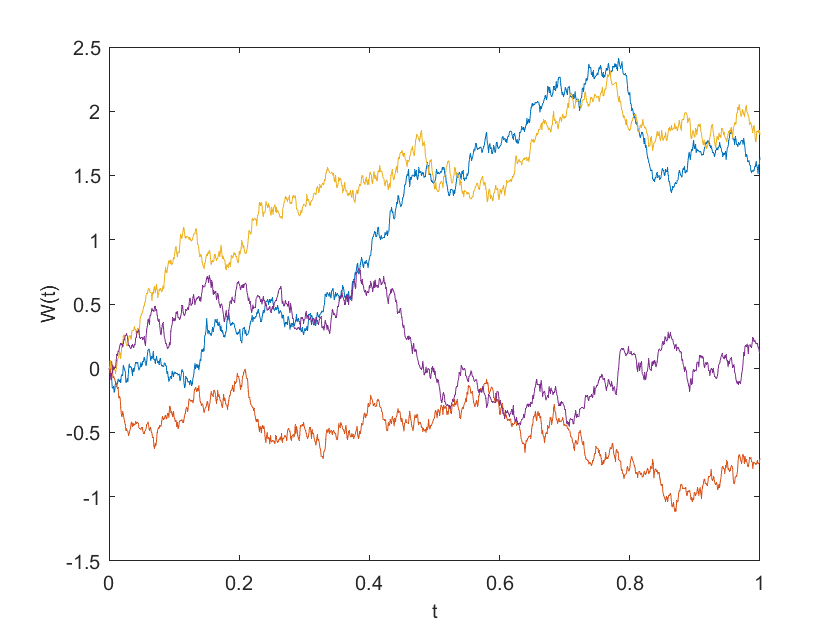
\includegraphics[width=0.8\textwidth]{figures/plot_bm.png}
    \end{figure}
  \end{block}
  

\end{column}

\separatorcolumn

\begin{column}{\colwidth}

  \begin{block}{Stochastic Integrals}
  
  \heading{Filtration} Increasing family of sub $\sigma$-algebras $\{\mathcal{F}_t\}$ of $\mathcal{F}$\\
       $\mathcal{F}_0  \subseteq \mathcal{F}_s  \subseteq \mathcal{F}_t  \subseteq \mathcal{F}$ if $0 \leq s \leq t$.
  \heading{Wiener Integral} \\
        \begin{itemize}
        \item Suppose $f$ is a step function given by $f = \sum_{i=1}^n a_i \cdot \mathbf{1}_{[t_{i-1}, t_i]}$, where $t_0 = 0$ and $t_n = T$. In this case, define 
        \[\mathbf{I}(f) = \int_0^{T}{f(t)\,dW_t} = \sum_{i=1}^n a_i \cdot W(t_i) - W(t_{i-1})\]
        where $f \in L^2[0,T]$ is a step process.

            \item Let $f \in L^2[0,T]$. The limit $\mathbf{I}(f) = \lim_{n \to \infty} \mathbf{I}(f_n)$ in $L^2(\Omega)$ is called the Wiener integral of $f$. The Wiener integral $\mathbf{I}(f)$ of $f$ will be denoted by:
\[ \mathbf{I}(f)(\omega) = \int_{0}^{T} f(t) \, dW(t)(\omega) \]
 where $f_n \in L^2[0,T]$ is a sequence of step process.
        \end{itemize}
        
        
         \heading{Properties of Wiener Integral} \\
         $\mathbf{I}(f) = \int_0^T f(t)\,dW_t$ is a \textbf{Normal Random variable} with mean $0$ and variance $\int_0^T f(t)^{2}\,dt$.
\begin{enumerate}
    \item $E[\int_0^T f(t)\,dW_t] = 0$.
    \item $E[(\int_0^T f(t)\,dW_t)^{2}] = \int_0^T f^{2}(t)\,dt$.
    \item Let $f \in L^2[0,T]$.Then the stochastic process \[ M_t = \int_0^t f(s)\,dW(s),\ 0 \leq t \leq T,\] is a \textbf{Martingale} with respect to $\mathcal{F}_t$, where $\mathcal{F}_t = \sigma\{W_s:0\leq s\leq t\}$.
\end{enumerate}
  \end{block}

  \begin{block}{It$\hat{\text{o}}$ Integral}

    \begin{itemize}
       \item Fix a Brownian motion $W(t)$ and filtration $\{ \mathcal{F}_t; \ 0 \leq t \leq T \}$ satisfying the following conditions:
       \begin{enumerate}
           \item For each $t$, $W(t)$ is $\mathcal{F}_t$-measurable.
           \item For any $s \leq t$, the random variable $W(t) - W(s)$ is independent of the $\sigma$-algebra $\mathcal{F}_s$.
       \end{enumerate}
       \item We will use $L_\text{ad}^2([0,T] \times \Omega)$ to denote the space of all stochastic process $f(t,\omega), \ 0 \leq t \leq T, \ \omega \in \Omega$ satisfying the following conditions:
       \begin{enumerate}
           \item $f(t,\omega)$ is adapted to the filtration $\{\mathcal{F}_t\}$.
           \item $\int_0^T{E({\left | f(t) \right |}^2)}\,dt < \infty$.
       \end{enumerate}
        \item \[f(t,\omega) = \sum_{i=1}^{n}{a_{i-1}(\omega)\mathbf{1}_{[t_{i-1},t_i]}(t)}\]
        \[\mathbf{I}(f) = \int_0^T f(t,\omega)\,dW_t(\omega) = \sum_{i=1}^n{a_{i-1}(W(t_i) - W(t_{i-1}))}\]
           \end{itemize}
        \heading{Properties of It$\hat{\text{o}}$ Integral} 
         $f \in L_\text{ad}^2([0,T] \times \Omega)$. $\mathbf{I}(f) = \lim_{n \rightarrow \infty}\mathbf{I}(f_n)$ where $\{f_n(t,\omega); \ n \geq 1\}$ is a sequence of adapted step stochastic process.
        \begin{enumerate}
            \item ${E}[\int_0^T f(t)\,dW] = 0$.
          \item ${E}[(\int_0^T f(t)\,dW_t)^{2}] = E[\int_0^T f^{2}(t)\,dt]$ 
          \item If $f \in L^2_\text{ad}[(0,T) \times \Omega]$, then the indefinite integral $\mathbf{I}(\cdot)$ is a \textbf{Martingale}. Furthermore, $\mathbf{I}(\cdot)$ has a version with continuous sample paths a.s.
        \end{enumerate}

 

  \end{block}
  
\begin{block}{It$\hat{\text{o}}$ formula}
 \begin{itemize}
     \item $X(\cdot)$ is a real-valued stochastic process satisfying \[ X(r) = X(s) + \int_s^r F\,dt + \int_s^r G\,dW\] for some $F \in L^1_\text{ad}[(0,T)\times \Omega], G \in L^2_\text{ad}[(0,T)\times \Omega]$ and all times $0 \leq  s \leq r \leq T$.We say that $X(\cdot)$ has the stochastic differential 
     \[ dX = F dt + G\,dW\] for $0 \leq t \leq T$
     \item $X(\cdot)$ has a stochastic differential \[ dX = F dt + G\,dW\] for $F \in L^1_\text{ad}[(0,T)\times \Omega], G \in L^2_\text{ad}[(0,T)\times \Omega]$.Assume $u \colon \mathbb{R} \times [0,T] \rightarrow \mathbb{R}, u = u(x,t)$ is continuous and that its partial derivatives $u_t = \frac{\partial u}{\partial t}, u_x = \frac{\partial u}{\partial x}$ and $u_{xx} = \frac{\partial^2 u}{\partial x^2}$  exist and are continuous.\\
     Then $Y(t) := u(X(t),t)$ has the stochastic differential 
     \begin{align*}
         \,du(X,t) &= u_t\,dt + u_x\,dX + \frac{1}{2} u_{xx} G^2\,dt\\
         &= (u_t + u_x F + \frac{1}{2} u_{xx} G^2)\,dt + u_x G\,dW
     \end{align*}
 \end{itemize}





    
\end{block}




\end{column}

\separatorcolumn

\begin{column}{\colwidth}

  \begin{block}{Stochastic Differential Equation}
    \[dX(t) = f(t,X(t))\,dt + \sigma(t,X(t))\,dW_t, \quad t \in (0,T) \]  \[X(0) = X_0 \quad  \dots \text{ (1)} \] 
    \[X(t) = X_0 + \int_0^t f(s,X(s))\,ds + \int_0^t \sigma(s,X(s))\,dW_s \quad \text{almost surely in} \ P.\]
    
    \heading{Definition of solution of SDE}
    A stochastic process $X \colon [0,T] \times \Omega \rightarrow \mathbb{R}$ is called a solution of the SDE (1) if
    \begin{itemize}
        \item $X(\cdot)$ is progressively measurable.(i.e. $X \colon [0,t] \times \Omega \rightarrow \mathbb{R} \text{ is } \mathcal{B}[0,t]\times\mathcal{F}_t$ measurable for all $t \geq 0$).
        \item $f(\cdot,X(\cdot)) \in L_{\text{ad}}^1([0,T] \times \Omega)$.
        \item $\sigma(\cdot,X(\cdot)) \in L_{\text{ad}}^2([0,T] \times \Omega)$.
        \item $\forall t \in [0,T],X(t)$ satisfies
        \[X(t) = X_0 + \int_0^t f(s,X(s))\,ds + \int_0^t \sigma(s,X(s))\,dW_s \quad \text{almost surely in} \ P.\]
    \end{itemize}


     \heading{Existence and Uniqueness Theorem}
    Let $f \colon [0,T] \times \mathbb{R} \rightarrow \mathbb{R}$ and $\sigma \colon [0,T] \times \mathbb{R} \rightarrow \mathbb{R}$ are continuous and for some $L > 0$ satisfies 
    \[ \left|f(t,x) - f(t,y)\right| \leq L\left|x-y\right|, \ \left|\sigma(t,x) - \sigma(t,y)\right| \leq L\left|x-y\right|\]
    \[ \left|f(t,x)\right| \leq L(1+\left|x\right|) ,\left|\sigma(t,x)\right| \leq L(1+\left|x\right|) \ \forall t \in [0,T], x \in \mathbb{R}\]
    Let $X_0 \colon \Omega \rightarrow \mathbb{R}$ be random variable, ${\E}\left|X_0\right|^2 < \infty $. Then, there exists a unique solution $X \in L^2_\text{ad}([0,T] \times \Omega)$ of SDE(1).

  \end{block}
  \begin{block}{Deterministic vs Stochastic Differential Equation}
  \begin{figure}[htbp]
  \centering
  \begin{subfigure}[b]{0.47\textwidth}
    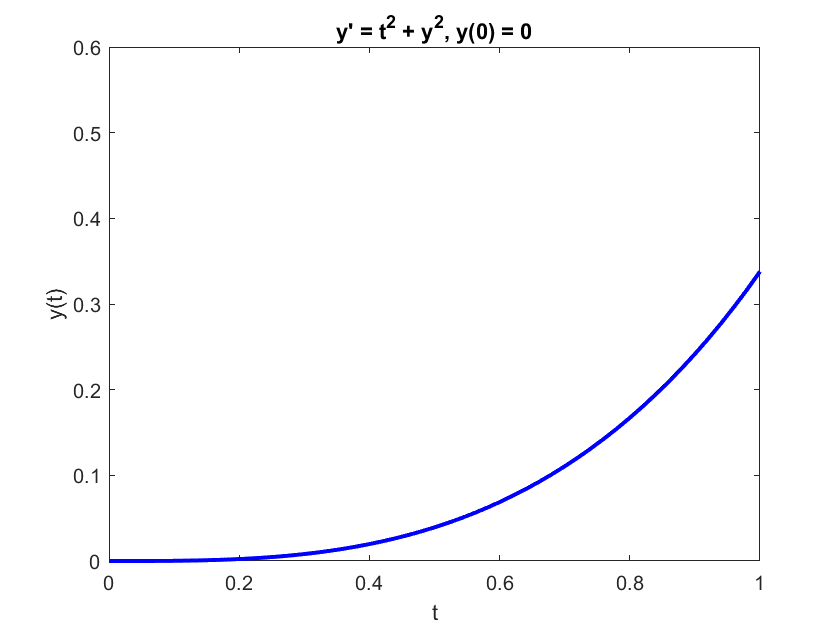
\includegraphics[width=\textwidth]{figures/deterministic_SDE.png}
    \caption{$\,dy(t) = (t^2 + y^2)\,dt$\\
    \textbf{Euler's scheme to solve the ODE:}
      \[\frac{dy}{dt} = f(t,y(t)),\ 0 \leq t \leq T\]
      \[y(0) = y_0\]
      is given by:
      \[\omega_0 = y_0\]
      \[\omega_{n+1} = \omega_n + hf(t_n,\omega_n),\]
      \[n=0,1,\dots,N-1\] 
      where $h=\frac{T}{N}, \ t_n = nh$
       }
    
    \label{fig:deterministic}
  \end{subfigure}
  \hfill
  \begin{subfigure}[b]{0.47\textwidth}
    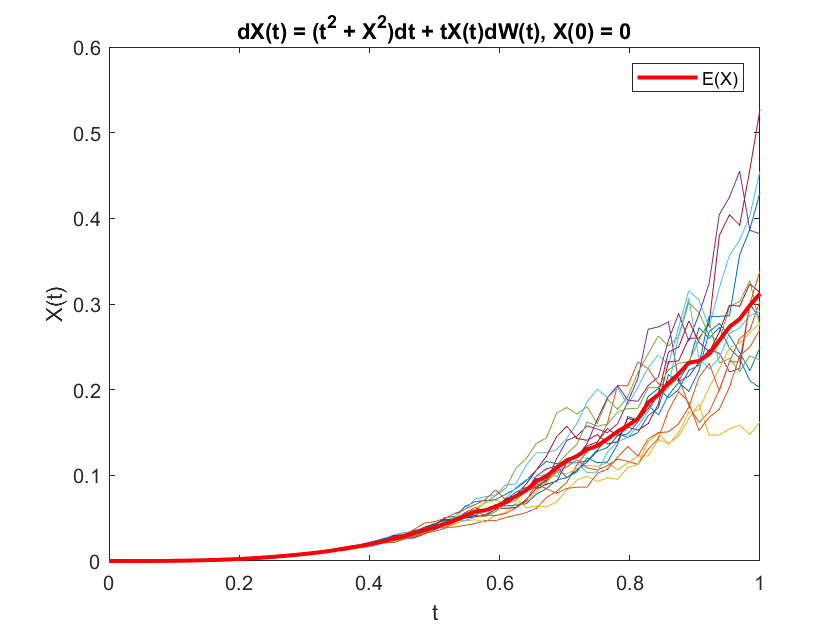
\includegraphics[width=\textwidth]{figures/stochastic_SDE.png}
    \caption{$\,dX(t) = (t^2 + X^2)\,dt + tX(t)\,dW(t)$
    \\ \textbf{Euler-Maruyama scheme to solve the SODE:}\\
      \[dX(t) = f(t,X(t))\,dt + \sigma(t,X(t))\,dW_t,\ 0 \leq t \leq T \]
      \[X(0) = X_0\]
      is given by:
      \[X_{n+1} = X_n + hf(t_n,X_n) + \sigma(t_n,X_n)\Delta dW_n,\]  \[n=0,1,\dots,N-1\]
      where $h=\frac{T}{N}, \ t_n = nh,$\\
      $ \Delta W_n = W(t_{n+1}) - W(t_n) \approx \sqrt{h}N(0,1)$
      
    }
    \label{fig:stochastic}
  \end{subfigure}
  %\caption{Main caption for the side-by-side plots}
  \label{fig: solution of SDE}
\end{figure}
  
      
  \end{block}

  \begin{exampleblock}{Examples}
    \begin{itemize}
        \item \textbf{Stock Price:}
        Let $S(t)$ denote the stock prices at time $t$. The evolution of $S(t)$ is given by the SDE: 
        \[\frac{d S(t)}{S(t)} = \mu\,dt + \sigma\,dW_t\]
        \[t > 0, \ S(0) = S_0, \ \mu > 0, \ \sigma \in \mathbb{R}\]
        \item \textbf{Brownian Bridge:}
        \[dB(t) = \frac{-B}{1-t}\,dt + \,dW_t\]
        \[0 < t < 1,\ B(0) = 0\]
        \item \textbf{Langevin's Equation:}
        \[\,dX(t) = -bX(t)\,dt + \sigma\,dW_t\]
        \[t > 0 , \ X(0) = X_0\]
       
    \end{itemize}


  \end{exampleblock}

  \begin{block}{References}
    \begin{itemize}
        \item \href{https://drive.google.com/file/d/1vRMD3PfWG5iZTjwdAeLyz3_fwPLslEyn/view?usp=drive_link}{Kuo H. H.,-Introduction to Stochastic Integration-Springer (2005)}
        \item \href{https://drive.google.com/file/d/1dDVWcERBHMOOmIBrovXGwt5KPLrIyRxC/view?usp=drive_link}{Oksendal B-Stochastic Differential Equations-Springer (2000)}
        \item \href{https://drive.google.com/file/d/1EiN6uab1nWAKvLPzE0VfQuoJ4vpF1bjM/view?usp=drive_link}{Evans L. C. - An Introduction to Stochastic Differential Equations (2014)}
    \end{itemize}

  \end{block}

\end{column}

\separatorcolumn
\end{columns}

\end{frame}

\end{document}
